\documentclass[compress]{beamer}
\usepackage{ifthen,verbatim}

\title{CMS: Alignment work and data flow}
\author{Jim Pivarski, Alexei Safonov}
\institute{Texas A\&M University}
\date{26 June, 2007}

\newcommand{\isnote}{}
\xdefinecolor{lightyellow}{rgb}{1.,1.,0.25}
\xdefinecolor{darkblue}{rgb}{0.1,0.1,0.7}

%% %% Uncomment this to get annotations
%% \def\notes{\addtocounter{page}{-1}
%%            \renewcommand{\isnote}{*}
%% 	   \beamertemplateshadingbackground{lightyellow}{white}
%%            \begin{frame}
%%            \frametitle{Notes for the previous page (page \insertpagenumber)}
%%            \itemize}
%% \def\endnotes{\enditemize
%% 	      \end{frame}
%%               \beamertemplateshadingbackground{white}{white}
%%               \renewcommand{\isnote}{}}

%% Uncomment this to not get annotations
\def\notes{\comment}
\def\endnotes{\endcomment}

\setbeamertemplate{navigation symbols}{}
\setbeamertemplate{headline}{\includegraphics[height=1 cm]{../cmslogo} \hspace{0.1 cm} \includegraphics[height=1 cm]{../tamulogo} \hfill
\begin{minipage}{5.5 cm}
\vspace{-0.75 cm} \small
\begin{center}
\ifthenelse{\equal{\insertpagenumber}{1}}{}{\textcolor{blue}{\insertsection}}
\end{center}
\end{minipage} \hfill
\begin{minipage}{4.5 cm}
\vspace{-0.75 cm} \small
\begin{flushright}
\ifthenelse{\equal{\insertpagenumber}{1}}{}{Jim Pivarski \hspace{0.5 cm} \insertpagenumber\isnote/\pageref{numpages}}
\end{flushright}
\end{minipage}\mbox{\hspace{0.2 cm}}}

\begin{document}
\frame{\titlepage}

\begin{notes}
\item This is the annotated version of my talk.
\item If you want the version that I am presenting, download the one
labeled ``slides'' on Indico (or just ignore these yellow pages).
\item The annotated version is provided for extra detail and a written
record of comments that I intend to make orally.
\item Yellow notes refer to the content on the {\it previous} page.
\item All other slides are identical for the two versions.
\end{notes}

\begin{notes}
\frametitle{Preliminary outline (won't appear in this form in the talk)}
\item \tiny General direction of this talk: physical data flow, software, monitoring, alignment exercises
\begin{itemize}
    \item \tiny Tracking systems at CMS
    \item \tiny Continuous alignment
\end{itemize}
\item \tiny Data flow
\begin{itemize}
    \item \tiny From CMS readout to alignment to corrected data
    \item \tiny Triggers, express stream
    \item \tiny Specialized AlCaReco data format
    \item \tiny Alignment time estimates
\end{itemize}
\item \tiny Software
\begin{itemize}
    \item \tiny Common framework for (a) all subdetectors and (b) all algorithms
    \item \tiny All tracking systems integrated: pixel, si-strips, muon barrel and endcap
    \item \tiny HIP, MillePede II, and Kalman
\end{itemize}
\item \tiny Monitoring
\begin{itemize}
    \item \tiny We foresee monitoring at four stages
    \item \tiny Both routine plots for shifter/aligners and expert tools for diagnostics
\end{itemize}
\item \tiny Alignment Exercises
\begin{itemize}
    \item \tiny CSA06: Computing Software Analysis Challenge '06
    \item \tiny CSA07: twice the computational load; more realistic
    \item \tiny Demonstration of complete tracker alignment with MillePede II
    \item \tiny Demonstration of muon chamber alignment with HIP
    \item \tiny Analysis of cosmic ray data underway: TIF and MTCC
\end{itemize}
\item \tiny Conclusion: Infrastructure for continuous alignment with lots of human
monitoring; full-scale exercises have proven principle, and cosmic-ray
alignments are underway
\end{notes}

\section*{Introduction}

\begin{frame}
\frametitle{General direction of this talk}
\begin{itemize}\setlength{\itemsep}{0.75 cm}
  \item Physical data flow: from raw data to alignment corrections
  \item Software architecture
  \item Monitoring alignment output
  \item Alignment exercises in Monte Carlo and data
\end{itemize}
\end{frame}

\begin{frame}
\frametitle{Tracking systems at CMS}
\begin{columns}
\column{0.5\linewidth}
\begin{center}
\includegraphics[height=3.5 cm]{tracker_leo.png}

Silicon tracker and pixel detector: 15,000 modules \\ \mbox{ }
\end{center}

\column{0.5\linewidth}
\begin{center}
\includegraphics[height=3.5 cm]{sun_shines_in_the_detector.jpg}

Muon detector: track sees 18--45 layers: an independent tracking system in its own right
\end{center}
\end{columns}

\vfill
\begin{itemize}
\item<2-> This talk will be both about alignment of both
\end{itemize}
\end{frame}

\section*{Physical data flow}

\begin{frame}
\begin{center}
\Huge \textcolor{blue}{Physical data flow}
\end{center}
\end{frame}

\begin{frame}
\frametitle{Motivation for prompt alignment}
\begin{itemize}\setlength{\itemsep}{0.75 cm}
\item CMS High-Level Trigger uses the same reconstruction software as offline, including alignment corrections

\item Alignment results improve the performance of our trigger

\item We want an infrastructure to immediately align on tracks, \\ as they are read out of the detector
\end{itemize}
\begin{center}
\includegraphics[width=8 cm]{readout.pdf}
\end{center}
\end{frame}

\begin{frame}
\frametitle{From CMS read-out to alignment to corrected data}
\begin{center}
\only<1>{\includegraphics[height=0.8\textheight]{grand_diagram5.pdf}}
\only<2>{\includegraphics[height=0.8\textheight]{grand_diagram4.pdf}}
\only<3>{\includegraphics[height=0.8\textheight]{grand_diagram3.pdf}}
\only<4>{\includegraphics[height=0.8\textheight]{grand_diagram2.pdf}}
\only<5>{\includegraphics[height=0.8\textheight]{grand_diagram1.pdf}}
\end{center}
\end{frame}

\begin{frame}
\frametitle{Triggers and Express Stream}
\begin{itemize}\setlength{\itemsep}{0.25 cm}
\item<1-> Both tracking systems use muons for alignment
\item<1-> Accept events from any trigger providing muons: \\ single $\mu$, di-$\mu$, $J/\psi$, $\Upsilon$, $Z \to \mu\mu$, $\mu$ with jets\ldots
\item<1-> Also include commissioning streams which select only on the basis of hardware trigger or partial High Level Trigger decisions

\vfill
\item<2-> Express Stream for alignment, calibration, monitoring, discovery channels (5--10\% in normal running, 25\% at first)
\item<2-> Alignment stream is filtered to include only tracks/hits used for alignment (3k/event tracker, 10k/event muon)
\end{itemize}
\end{frame}

\begin{frame}
\frametitle{Before first collisions}
\vspace{-1 cm}
\begin{columns}
\column{0.5\linewidth}
\begin{center}
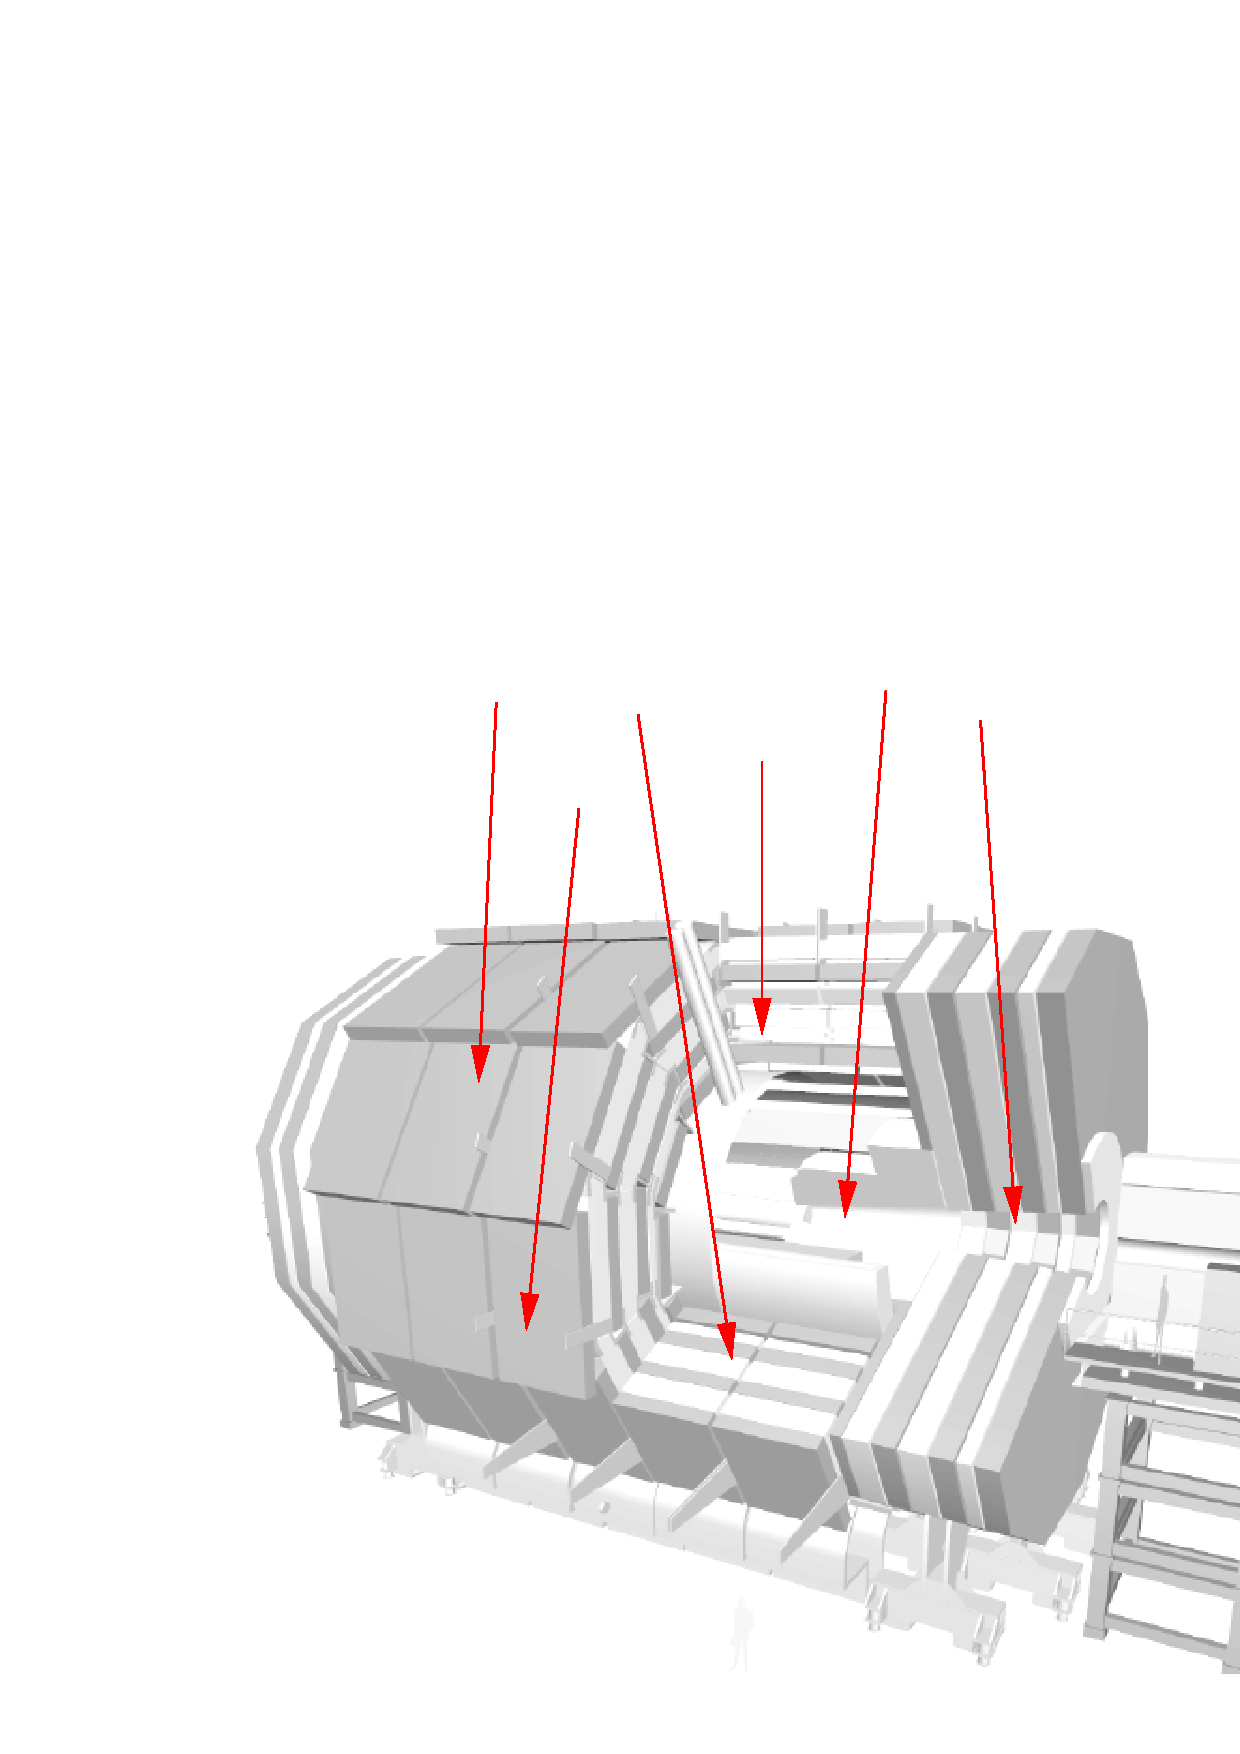
\includegraphics[height=3.5 cm]{cosmics.pdf}

Cosmic rays, especially for barrels
\end{center}

\column{0.5\linewidth}
\begin{center}
\includegraphics[height=3.5 cm]{beamhalo.pdf}

Beam-halo, especially for endcaps
\end{center}
\end{columns}

\vfill
\begin{itemize}
\item A special pair of scintillator paddles added to extend
$\eta$ range of beam-halo trigger for tracker
\end{itemize}
\end{frame}

\section*{Software}

\begin{frame}
\begin{center}
\Huge \textcolor{blue}{Software}
\end{center}
\end{frame}

\begin{frame}
\frametitle{Common framework}
\begin{itemize}
\item Common framework for
\begin{enumerate}[(\alph{enumi}) ]
\item all subdetectors
\begin{itemize}
\item Muon system and Si-tracker use the same tracking data-formats and fitting algorithms
\end{itemize}

\item all algorithms
\begin{itemize}
\item HIP, MillePede II, and Kalman are plug-in modules
\end{itemize}
\end{enumerate}

\vfill
\item Centrally manages
\begin{itemize}
\item hierarchical geometry description with uncertainties and correlations at each level
\item coordinate transformations and derivatives
\item fixing/floating components and parameters
\item application of survey constraints
\item database access
\end{itemize}
\end{itemize}
\end{frame}

\begin{frame}
\frametitle{Built-in parallel-processing}
\begin{itemize}
\item Large alignment job can be split into sub-jobs
\item Sub-jobs store partial calculations in temporary ROOT files
\item JobCollector merges partial results, performs final calculation
\item Monitoring histograms are merged in the same way

\vfill
\begin{center}
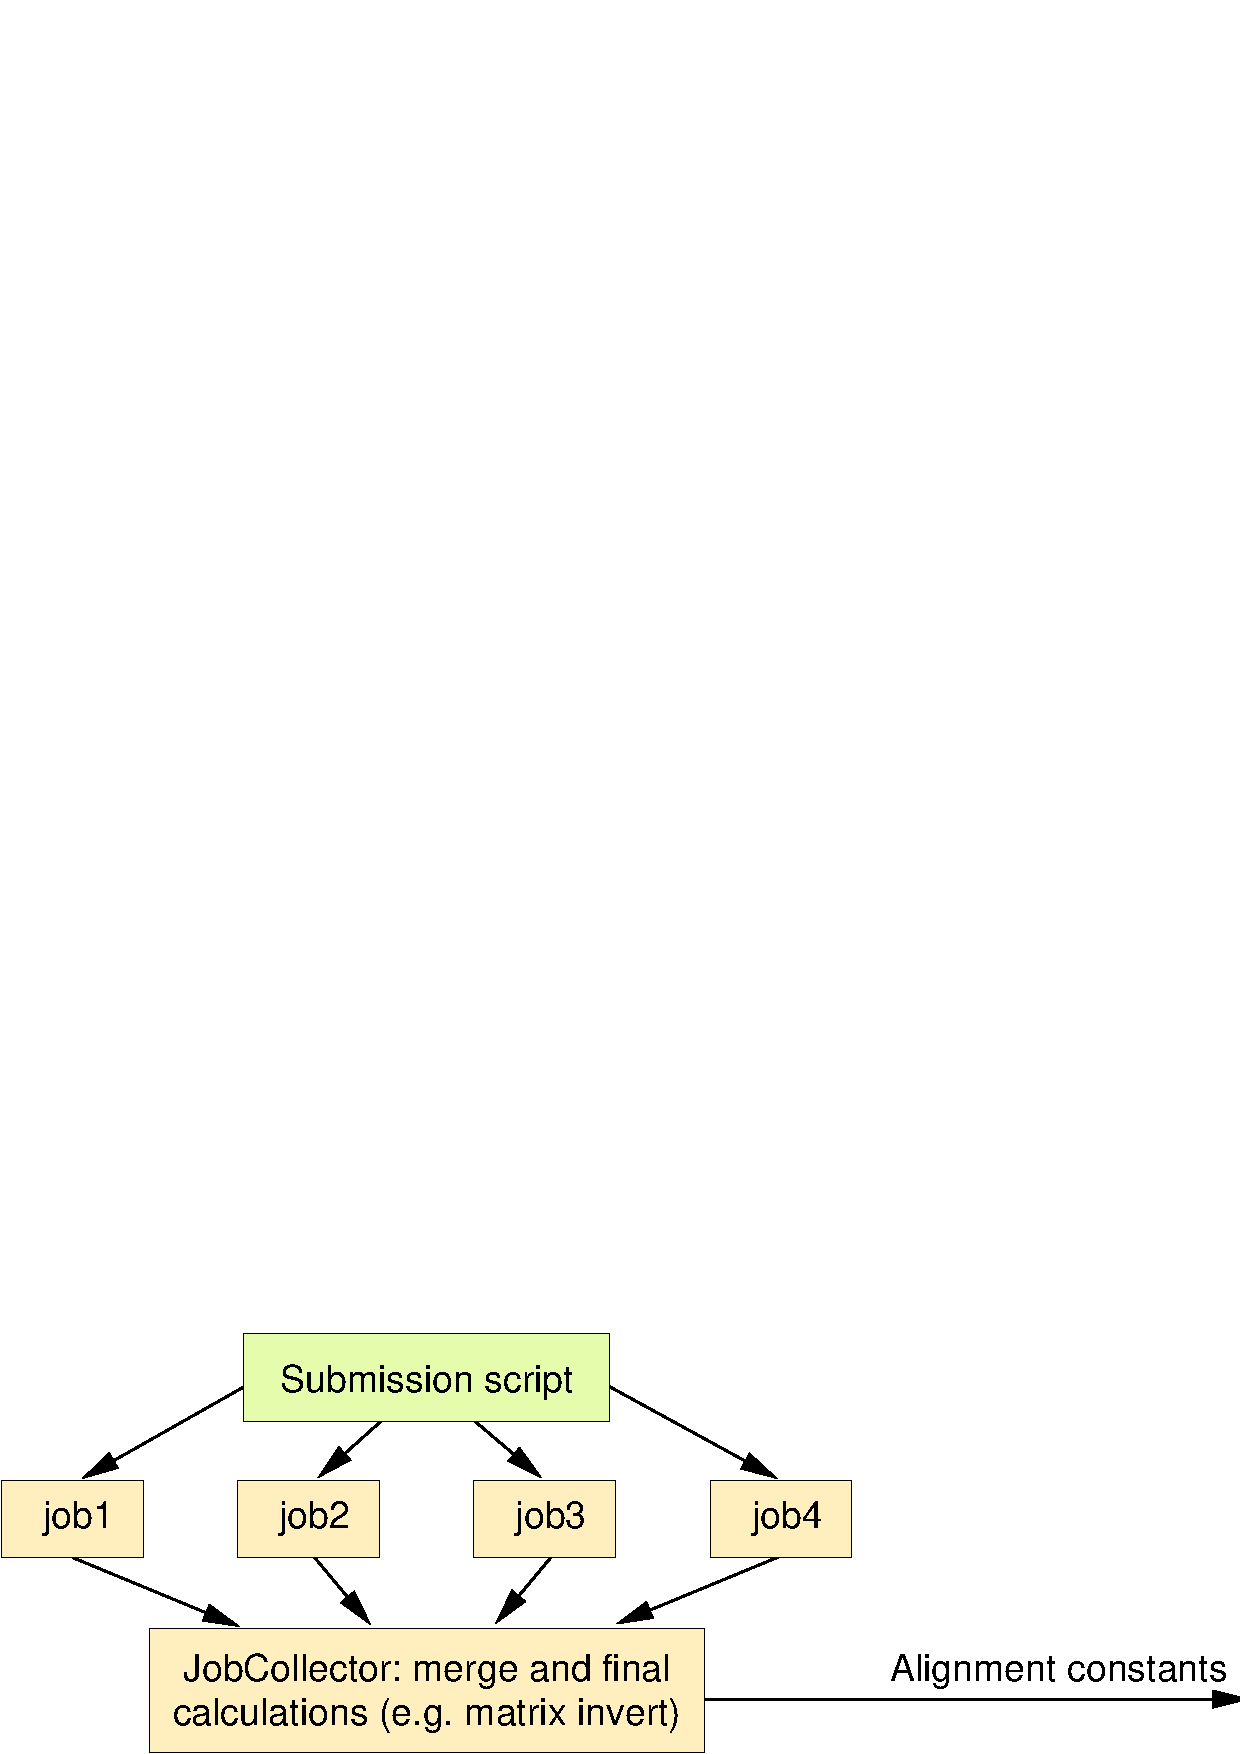
\includegraphics[width=0.8\linewidth]{jobcollector.pdf}
\end{center}

\vfill
\item Total time is determined by the last sub-job to finish, so
alignment requires a dedicated farm
\end{itemize}
\end{frame}

\section*{Monitoring}

\begin{frame}
\begin{center}
\Huge \textcolor{blue}{Monitoring}
\end{center}
\end{frame}

\begin{frame}
\frametitle{Four stages of monitoring}
\begin{enumerate}[(\alph{enumi}) ]\setlength{\itemsep}{0.75 cm}
\item Specialized plots for shifters in Data Quality Monitor \\ (e.g.\ $Z$ peak, agreement between overlapping chambers)
\item Monitoring plots built into the alignment process
\item Non-event level comparison of alignment geometries \\ (``how
different are these geometries?''), comparison with hardware/survey, and
as a function of time
\item Last check that we put the right thing into the database \\
(same plots as \textcolor{darkblue}{(a)})
\end{enumerate}
\end{frame}

\begin{frame}
\frametitle{Four stages of monitoring}
\begin{center}
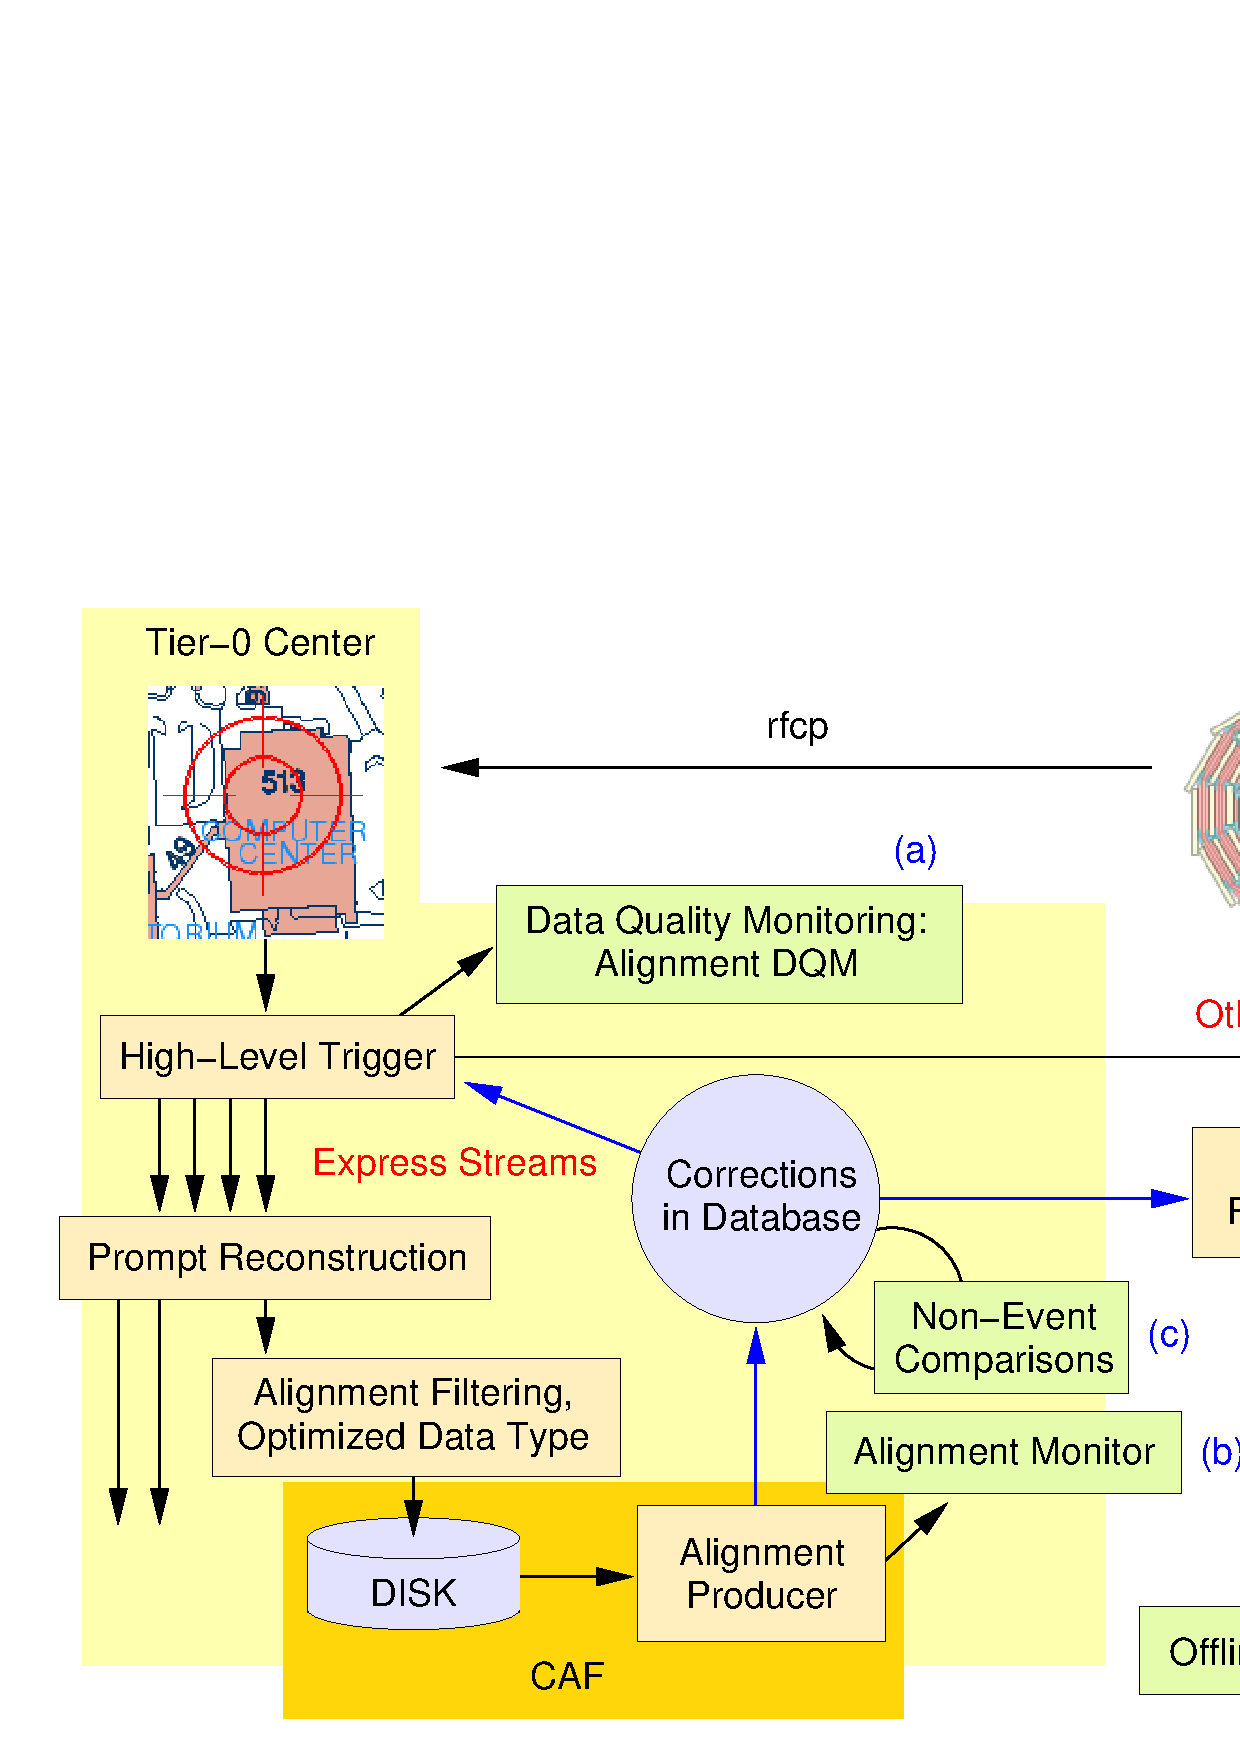
\includegraphics[height=0.8\textheight]{grand_diagram0.pdf}
\end{center}
\end{frame}

\begin{frame}
\frametitle{Expert systems and routine plots}
\begin{itemize}
\item Expert systems
\begin{itemize}
\item Discover and zoom into problem areas
\item Manually read alignment corrections off of profiles
\end{itemize}

\vfill
\includegraphics[width=\linewidth]{monitoring_tool.png}

\vfill
\item Routine plots
\begin{itemize}
\item Concise set of powerful alignment indicators
\item Will be derived from experience with expert systems
\end{itemize}
\end{itemize}
\end{frame}

%% \begin{frame}
%% \frametitle{$\chi^2$-invariant deformations}
%% \begin{center}
%% \includegraphics[width=0.7\linewidth]{chi2_invariants.png}
%% \end{center}
%% I should say something about this
%% \end{frame}

\section*{Alignment Exercises}

\begin{frame}
\begin{center}
\Huge \textcolor{blue}{Alignment Exercises}
\end{center}
\end{frame}

\begin{frame}
\frametitle{CSA06: Computing Software Analysis 2006}
\begin{itemize}
\begin{columns}
\column{0.6\linewidth}
\item $\frac{1}{4}$ of anticipated 2008 data
\item Emphasis on computing and work-flow, rather than \\ alignment quality
\column{0.35\linewidth}
\mbox{\hspace{-2 cm}}\includegraphics[width=1.35\linewidth]{csa06_tracker_results.png}\hspace{-1 cm}
\end{columns}
\item Full simulation of Si-tracker alignment
\begin{itemize}
\item 2 million misaligned $Z\to\mu\mu$
\item HIP algorithm on a prototype of the alignemnt farm
\item Read/wrote geometry from database on-the-fly
\item Event sample re-reconstructed with corrections
\end{itemize}

\vfill
\item Muon alignment tested the possibility of aligning at a remote
Tier-2 site, with a simplified MillePede II algorithm
\end{itemize}
\end{frame}

\begin{frame}
\frametitle{CSA\textcolor{blue}{07}}
\begin{itemize}\setlength{\itemsep}{0.5 cm}
\item Twice the data
\item Mixed sample selected by High Level Trigger for realism
\item Filter using simple $p_T$ cut and using di-$\mu$ mass
\item Tracker alignment will use the full MillePede II algorithm
\item Muon alignment will do a full simulation with HIP \\
(analogous to tracker in CSA06)
\item Full exercise starts September 15
\end{itemize}
\end{frame}

\begin{frame}
\frametitle{Demonstration of complete MillePede II tracker alignment}
\begin{center}
\begin{tabular}{p{0.45\linewidth} p{0.45\linewidth}}
\includegraphics[width=\linewidth]{tracker_alignment_milestone1.png} &
\includegraphics[width=\linewidth]{tracker_alignment_milestone2.png}
\end{tabular}
\end{center}
\begin{itemize}

\vspace{-0.5 cm}
\item 2 GB RAM, 1 h 40 min CPU (10 min matrix inversion)
\item 3.5 million muon tracks
\end{itemize}
\end{frame}

\begin{frame}
\frametitle{Demonstration of muon chamber alignment}
\begin{enumerate}[(\alph{enumi}) ]
\item align muon system \textcolor{blue}{to tracker}
\item align \textcolor{red}{standalone} muon system without external reference
\end{enumerate}
\begin{center}
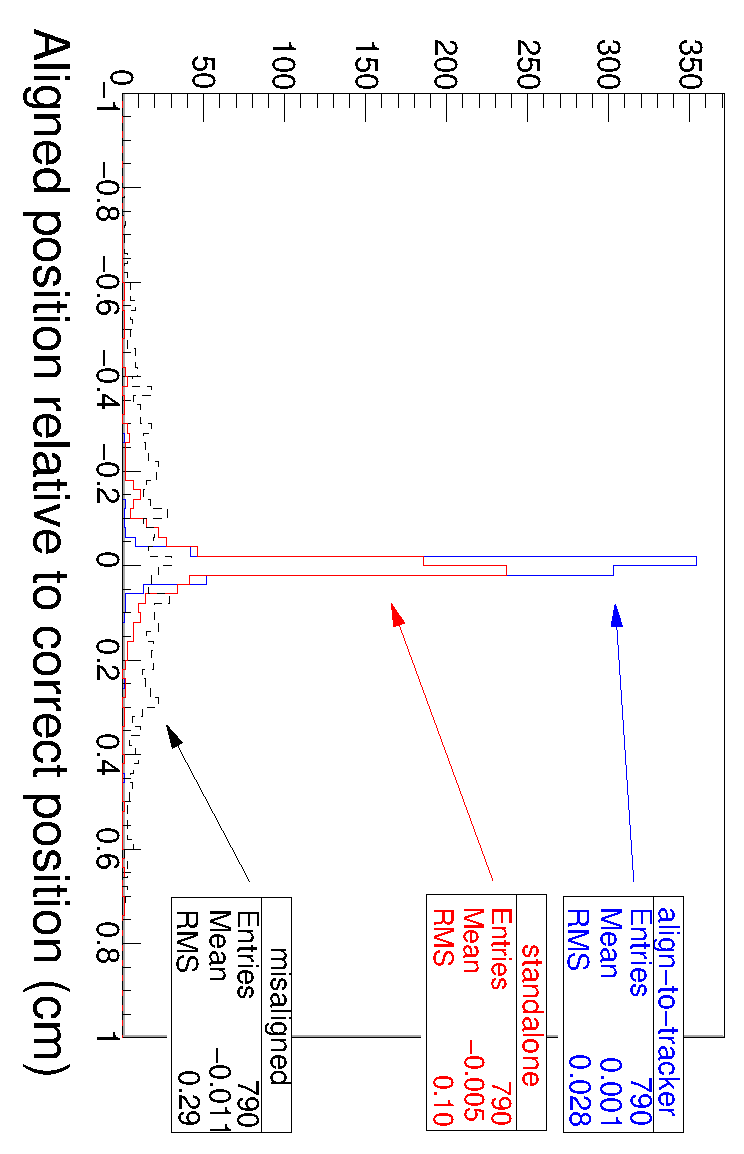
\includegraphics[height=0.6\linewidth, angle=90]{x_positions}
\end{center}
\begin{itemize}
\item 6 degrees of freedom, realistic initial misalignment
\item 30 min per iteration (only \textcolor{red}{standalone} requires iterations)
\item 16,000 muon tracks
\end{itemize}
\end{frame}

\begin{frame}
\frametitle{Analysis of cosmic ray data underway}
\begin{itemize}
\item<1-> 25\% of Si-tracker is taking data in the Tracker Integration Facility (b\^at 186)
\item<1-> 2 million cosmic rays (2 months)
\item<1-> All three algorithms are currently being applied

\vfill
\item<2-> 21 muon chambers collected data in last September's \\
Magnet Test Cosmics Challenge
\item<2-> HIP and MillePede II are currently being applied

\vfill
\item<3-> Real-data alignment efforts will continue with cosmic rays
from upcoming Slice Tests, Global-Running-at-End-of-Months, local
cosmic runs, and beam-halo from beam commissioning
\end{itemize}
\end{frame}

\section*{Conclusions}

\begin{frame}
\frametitle{Conclusions}
\begin{itemize}\setlength{\itemsep}{0.75 cm}
\item Infrastructure (farms, data streams) under development for prompt alignment
\item Opportunities for human monitoring
\item Proof-of-principle with full-scale exercises
\item Cosmic ray alignments are happening right now
\end{itemize}
\label{numpages}
\end{frame}

\end{document}

%%%%%%%%%%%%%%%%%%%%%%%%%%%%%%%%%%%%%%%%%%%%%%%%%%%%%%%%%%%%%%%%%%%%%%%%%%%%%%%%%%%%%%%%%%%

%% \begin{frame}
%% \frametitle{information dump}
%% \begin{center}
%% \includegraphics[height=0.8\textheight]{alexeis_graph2.png}
%% \end{center}
%% \end{frame}

%% \begin{frame}
%% \frametitle{information dump}
%% \begin{itemize}
%% \item IP5 $\to$ $\to$ $\to$ rfcp transfer $\to$ $\to$ $\to$ T0 centre
%% (CASTOR2 disk), CAF (Central Analysis Facility) 50-150 TB
%% \item All muon triggers (single isolated $\mu$, single relaxed $\mu$,
%% double relaxed $\mu\mu$, $J/\psi \to \mu\mu$, $\Upsilon \to \mu\mu$,
%% $Z \to \mu\mu$, triple relaxed $\mu\mu\mu$, same-sign double
%% $\mu^\pm\mu^\pm$
%% \item Commissioning triggers which select on the basis of only L1, L2:
%% we'll take these, too
%% \item Express stream (25\% of data at first, later tightened to
%% 5--10\%): $Z$, $W\to\mu\nu$, $J/\psi$, $\Upsilon$
%% \item CAF: T0 $\to$ prompt reco $\to$ stripped to AlCaReco format
%% \item $\mu$ AlCaReco is 40 kB/event
%% \item (CMS to RTAG document says this is 10$\times$ too much?!?)
%% \end{itemize}
%% \end{frame}

%% \begin{frame}
%% \frametitle{outline}
%% \begin{itemize}
%% \item \tiny General remarks; introduction
%% \item \tiny Data flow
%% \begin{itemize}
%% \item \tiny Step through the process from CMS readout to alignment on the
%% CAF to the database to corrected data
%% \item \tiny Express stream, triggers
%% \item \tiny Specialized AlCaReco data format
%% \item \tiny Alignment time estimates (supported by simulations)
%% \end{itemize}
%% \item \tiny Alignment software
%% \begin{itemize}
%% \item \tiny Common framework for (a) all subdetectors and (b) all algorithms
%% \item \tiny Tracker, Muon (say \#alignables each) implemented, ECAL, HCAL in development
%% \item \tiny HIP, MillePede II, and Kalman
%% \item \tiny Tracker: key HIP and MillePede results
%% \item \tiny Muon: HIP results
%% \begin{itemize}
%% \item \tiny Two approaches: align to tracker (1 iteration), self-alignment (7 iterations)
%% \end{itemize}
%% \item \tiny Application of survey constraints
%% \item \tiny Application of alignment parameter errors
%% \end{itemize}
%% \item \tiny Monitoring the output
%% \begin{itemize}
%% \item \tiny We foresee monitoring at 4 stages
%% \begin{itemize}
%% \item \tiny Specialized plots in Data Quality Monitor (DQM)
%% \item \tiny Monitoring plots built into the alignment process
%% \item \tiny Non-event level comparison of alignment geometries (``are they
%% {\it different?}''), comparison with hardware/survey, as a function of time
%% \item \tiny Last check that we put the right thing into the database
%% \end{itemize}
%% \item \tiny Both routine Shifter/Aligner plots and expert tools
%% \end{itemize}
%% \item \tiny Conclusion: we need regular routines, but also the potential for
%% human intervention at every stage
%% \end{itemize}
%% \end{frame}

